\documentclass[tikz, border=10pt]{standalone}
\usetikzlibrary{shapes.geometric, arrows.meta, positioning, calc}

\begin{document}

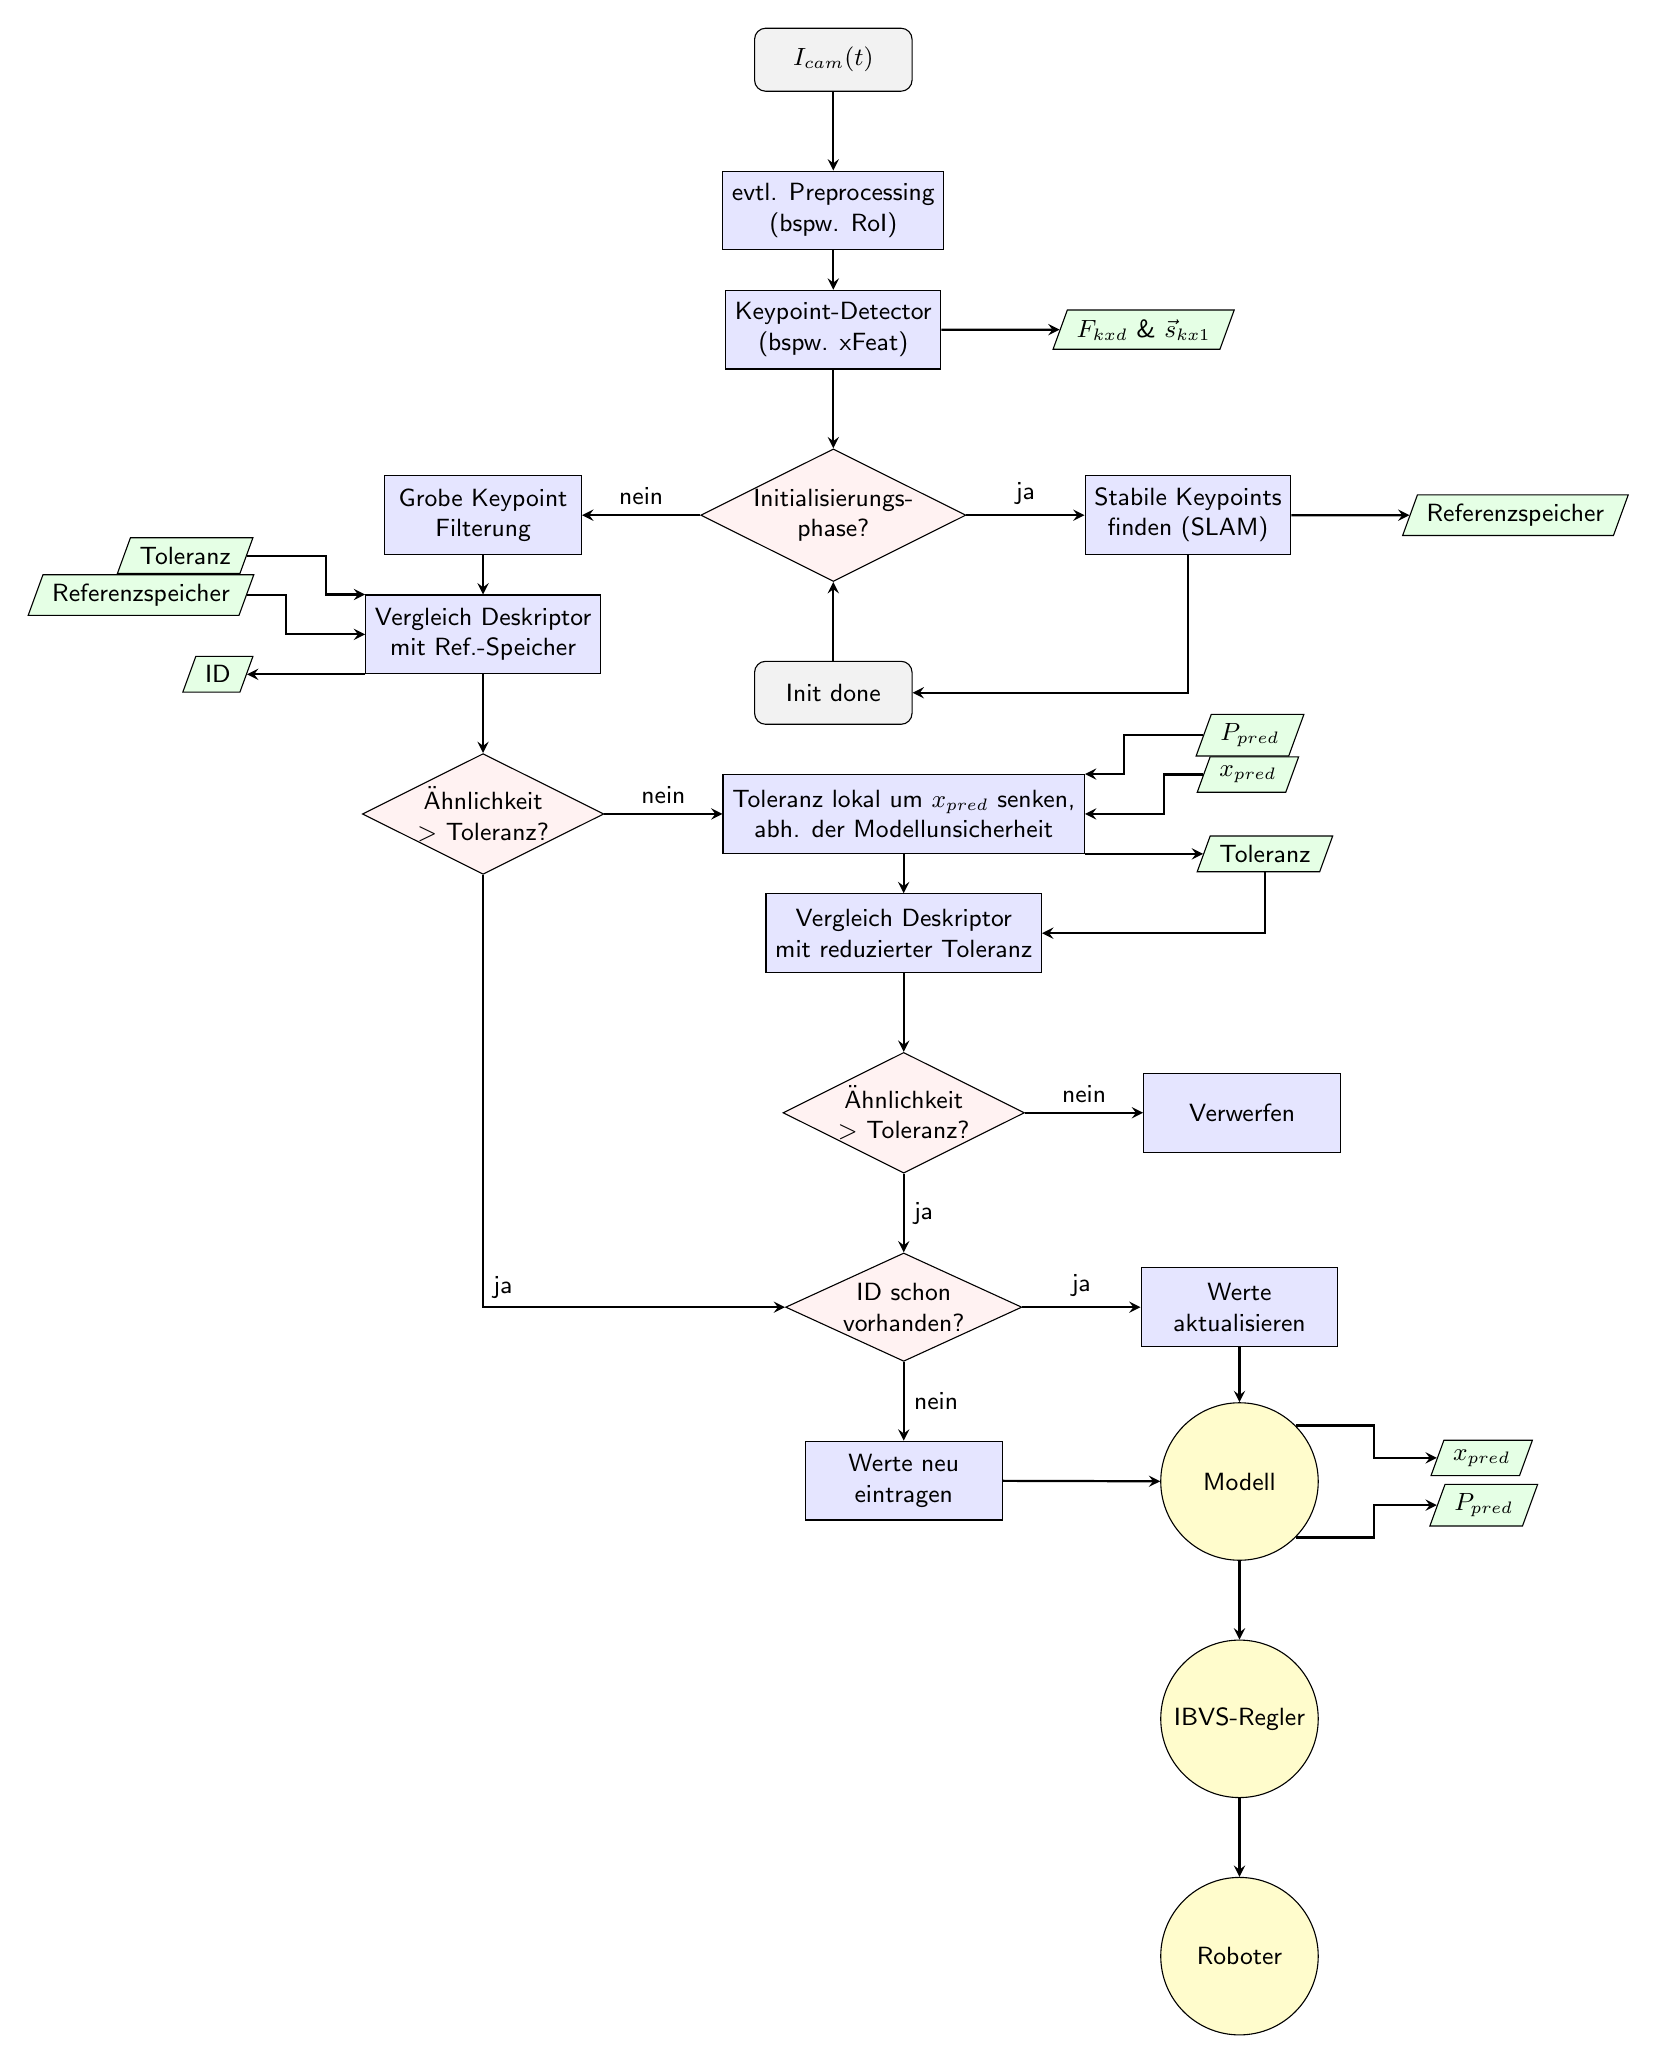
\begin{tikzpicture}[
    node distance=1cm and 1.5cm,
    font=\sffamily\small,
    % Styles für die verschiedenen Formen
    startstop/.style={rectangle, rounded corners, draw, fill=gray!10, minimum width=2cm, minimum height=0.8cm, align=center},
    process/.style={rectangle, draw, fill=blue!10, minimum width=2.5cm, minimum height=1cm, align=center},
    decision/.style={diamond, draw, fill=red!5, aspect=2, inner sep=0pt, minimum width=3cm, align=center},
    data/.style={trapezium, draw, trapezium left angle=70, trapezium right angle=110, fill=green!10, align=center},
    storage/.style={parallelogram, draw, fill=orange!10, minimum width=2cm, align=center},
    % subprocess/.style={circle, draw, fill=yellow!20, minimum size=1.5cm, align=center};
    arrow/.style={thick, ->, >=stealth}
]

% --- Ebene 1: Input & Keypoints ---
\node (input) [startstop] {$I_{cam}(t)$};
\node (preproc) [process, below=of input] {evtl. Preprocessing\\(bspw. RoI)};
\node (keypoint) [process, below=0.5cm of preproc] {Keypoint-Detector\\(bspw. xFeat)};
\node (feat_vec) [data, right=of keypoint] {$F_{kxd}$ \& $\vec{s}_{kx1}$};

% --- Ebene 2: Initialisierung vs. Tracking ---
\node (init_check) [decision, below=of keypoint] {Initialisierungs-\\phase?};
\node (stable_kp) [process, right=of init_check] {Stabile Keypoints\\finden (SLAM)};
\node (ref_store) [data, right=of stable_kp] {Referenzspeicher};
\node (init_done) [startstop, below=of init_check] {Init done};

% --- Ebene 3: Filterung & Vergleich ---
\node (kp_filter) [process, left=of init_check] {Grobe Keypoint\\Filterung};
\node (desc_comp) [process, below=0.5cm of kp_filter] {Vergleich Deskriptor\\mit Ref.-Speicher};
\node (ref_access) [data, left=of desc_comp, yshift=0.5cm] {Referenzspeicher};
\node (tol_access) [data, left=of desc_comp, yshift=1cm] {Toleranz};
\node (id_store) [data, left=of desc_comp.south west] {ID};

% --- Ebene 4: Deskriptor Logik ---
\node (desc_tol) [decision, below=of desc_comp] {Ähnlichkeit\\$>$ Toleranz?};

% --- Ebene 4.1: Local Rescue ---
\node (lr) [process, right=of desc_tol] {Toleranz lokal um $x_{pred}$ senken,\\abh. der Modellunsicherheit};
\node (x_access) [data, right=of lr, yshift=0.5cm] {$x_{pred}$};
\node (P_access) [data, right=of lr, yshift=1cm] {$P_{pred}$};
\node (tol_lr_store) [data, right=of lr.south east] {Toleranz};
\node (desc_comp_lr) [process, below=0.5cm of lr] {Vergleich Deskriptor\\mit reduzierter Toleranz};
\node (desc_tol_2) [decision, below=of desc_comp_lr] {Ähnlichkeit\\$>$ Toleranz?};
\node (discard) [process, right=of desc_tol_2] {Verwerfen};

% --- Ebene 4.2: passt ---
\node (id_exists) [decision, below=of desc_tol_2] {ID schon\\vorhanden?};
\node (update_vals) [process, right=of id_exists] {Werte\\aktualisieren};
\node (entry_vals) [process, below=of id_exists] {Werte neu\\eintragen};

% --- Ebene 5: Modell ---
% \node (Modell) [subprocess, below=of update_vals, yshift=-0.19cm] {Modell};
\node (modell) [circle, draw, fill=yellow!20, minimum size=2cm, below=of update_vals, yshift=0.3cm] {Modell};
\node (x_store) [data, right=of modell, yshift=0.3cm] {$x_{pred}$};
\node (P_store) [data, right=of modell, yshift=-0.3cm] {$P_{pred}$};

% --- Ebene 6: Regler/Roboter ---
\node (regler) [circle, draw, fill=yellow!20, minimum size=2cm, below=of modell] {IBVS-Regler};
\node (robot) [circle, draw, fill=yellow!20, minimum size=2cm, below=of regler] {Roboter};


% --- Verbindungen ---
\draw [arrow] (input) -- (preproc);
\draw [arrow] (preproc) -- (keypoint);
\draw [arrow] (keypoint) -- (feat_vec);
\draw [arrow] (keypoint) -- (init_check);

\draw [arrow] (init_check) -- node[anchor=south] {ja} (stable_kp);
\draw [arrow] (stable_kp) -- (ref_store);
\draw [arrow] (init_check) -- node[anchor=south] {nein} (kp_filter);
\draw [arrow] (stable_kp) |- (init_done);
\draw [arrow] (init_done) -- (init_check);

\draw [arrow] (kp_filter) -- (desc_comp);
\draw [arrow] (desc_comp) -- (desc_tol);
\draw [arrow] (tol_access.east) -- ++(1,0) |- (desc_comp.north west);
\draw [arrow] (ref_access.east) -- ++(0.5,0) |- (desc_comp.west);
\draw [arrow] (desc_comp.south west) -- (id_store.east);

\draw [arrow] (desc_tol) -- node[anchor=south] {nein} (lr);
\draw [arrow] (desc_tol.south) |- node[anchor=west, yshift=0.25cm] {ja} (id_exists);

\draw [arrow] (x_access.west) -- ++(-0.5,0) |- (lr.east);
\draw [arrow] (P_access.west) -- ++(-1,0) |- (lr.north east);
\draw [arrow] (lr.south east) -- (tol_lr_store.west);
\draw [arrow] (lr) -- (desc_comp_lr);
\draw [arrow] (tol_lr_store.south) |- (desc_comp_lr.east);
\draw [arrow] (desc_comp_lr) -- (desc_tol_2);
\draw [arrow] (desc_tol_2) -- node[anchor=south] {nein} (discard);
\draw [arrow] (desc_tol_2) -- node[anchor=west] {ja} (id_exists);

\draw [arrow] (id_exists) -- node[anchor=south] {ja} (update_vals);
\draw [arrow] (id_exists) -- node[anchor=west] {nein} (entry_vals);

\draw [arrow] (entry_vals) -- (modell);
\draw [arrow] (update_vals) -- (modell);

\draw [arrow] (modell.north east) -- ++(1,0) |- (x_store.west);
\draw [arrow] (modell.south east) -- ++(1,0) |- (P_store.west);

\draw [arrow] (modell.south) -- (regler);
\draw [arrow] (regler) -- (robot);

\end{tikzpicture}
\end{document}